\documentclass{article}

\usepackage[letterpaper]{geometry}
\usepackage{amsmath}
\usepackage{amssymb}
\usepackage{graphicx}

\title{2231 Final Exam}
\author{Duncan Wilkie}
\date{9 December 2021}

\begin{document}

\maketitle

\section*{1a}
The field can be expected to be radial. Therefore, we may apply Gauss's law to find the field. The charge enclosed by a Gaussian surface consisting of a sphere of radius $r$ ($<R$) concentric with the charge distribution is
\[Q_{enc}=\int\rho(r)dV=\int_0^\pi\int_0^{2\pi}\int_0^r(ar)r^2\sin\varphi drd\theta d\varphi=4\pi a\int_0^rr^3dr=\pi ar^4\]
From Gauss's law,
\[\int\vec{E}\cdot d\vec{A}=\frac{Q_{enc}}{\epsilon_0}\Rightarrow 4\pi r^2|\vec{E}|=\frac{\pi ar^4}{\epsilon_0} \Leftrightarrow |\vec{E}|=\frac{ar^2}{4\epsilon_0} \Rightarrow \vec{E}=\frac{ar^2}{4\epsilon_0}\hat{r}\]

\section*{1b}
Outside the sphere, the same presumptions hold, but the enclosed charge integral stops at the radius of the sphere (call it $R$), so \[Q_{enc}=\pi aR^4\]
Applying Gauss's law,
\[4\pi r^2|\vec{E}|=\frac{\pi aR^4}{\epsilon_0} \Leftrightarrow |\vec{E}|=\frac{a R^4}{4\epsilon_0 r^2}\Rightarrow \vec{E}=\frac{aR^4}{4\epsilon_0 r^2}\hat{r}\]

\section*{1c}
The total charge of the sphere was calculated in part b to be $\pi aR^4$

\section*{1d}
The electric potential is by definition
\[V=-\int_{\mathcal{O}}^r\vec{E}\cdot d\vec{l}=-\int_{\infty}^0|\vec{E}(r)|dr=\int_{R}^\infty\frac{aR^4}{4\epsilon_0 r^2}dr+\int_0^R\frac{ar^2}{4\epsilon_0}dr\]
\[=\frac{aR^4}{4\epsilon_0}\left( -\frac{1}{3r^3}\bigg|_{R}^\infty \right)+\frac{a}{4\epsilon_0}\left( \frac{r^3}{3}\bigg|_0^R \right)=\frac{aR}{12\epsilon_0}+\frac{aR^3}{12\epsilon_0}\]

\section*{2a}
The general form of the multipole expansion of the potential resulting from a charge distribution is
\[V(\vec{r})=\frac{1}{4\pi\epsilon_0}\sum_{n=0}^\infty\frac{1}{r^{n+1}}\int (r')^nP_n(\cos\alpha)\rho(\vec{r'})dV\]
For this charge distribution, this is written with azimuthal coordinate correspondence $(r,\theta)$ and $(r',\vartheta)$ as
\[V(\vec{r})=\frac{1}{4\pi\epsilon_0}\sum_{n=0}^\infty\frac{1}{r^{n+1}}\left( \int_0^R\int_0^{\pi}(r')^n\lambda P_n(\cos[\vartheta-\theta])r'dr'd\vartheta-\int_0^R\int_\pi^{2\pi}(r')^n\lambda P_n(\cos[\vartheta-\theta])r'dr'd\vartheta\right)\]
\[=\frac{1}{4\pi\epsilon_0}\sum_{n=0}^\infty\frac{\lambda R^{n+2}}{(n+2)r^{n+1}}\left( \int_0^\pi P_n(\cos[\vartheta-\theta])d\vartheta -\int_\pi^{2\pi}P_n(\cos[\vartheta-\theta])d\vartheta\right)\]
The monopole term corresponds to $n=0$, whereupon $P_0(\cos[\vartheta-\theta])=1$ and the two integral terms are both $\pi$ and subtract to zero. Therefore, the monopole term is zero.

\section*{2b}
The dipole moment is by definition
\[\vec{p}=\int\vec{r'}\rho(\vec{r'})dV=\int_0^R\int_0^{2\pi}\vec{r'}\rho(\vec{r'})r'dr'd\theta=\hat{r'}\int_0^R(r')^2\left( \int_0^\pi\lambda d\vartheta-\int_\pi^{2\pi}\lambda d\vartheta\right)dr'=0\]

\section*{3a}
The bound volume charge is, since the polarization is constant,
\[\rho_b=-\nabla\times \vec{P}=0\]
The bound surface charge is
\[\sigma_b=\vec{P}\cdot\hat{n}\]
Presuming the axis of the cylinder is along the $z$-axis, the surface charge density on the non-circular face of the cylinder is zero, since $P\hat{z}$ is perpendicular to the unit normal vector to the face. For the circular faces, the polarization is parallel and antiparallel to the unit normal vector for the upper and lower face, respectively. Therefore, $\sigma_b=P$ for the upper face and $\sigma_b=-P$ for the lower face.

\section*{3b}
The total bound charge is the sum of the integrals of the volume charge density over the volume and the surface charge density over the surfaces:
\[Q_b=\int\rho_bdV+\int\sigma_b\cdot d\vec{A}\]The volume charge density, and therefore the volume charge integral, are zero. The only nonzero-surface-charge-density regions are at the caps of the cylinder, and since they are constants the charges are just $q_u=\pi R^2P$ and $q_l=-\pi R^2P$ for the upper and lower caps respectively. The sum of these two charges is zero, so the total bound charge is zero.

\section*{3c}
This is approximately the field due to two equally-and-oppositely-charged infinitely long sheets.
\[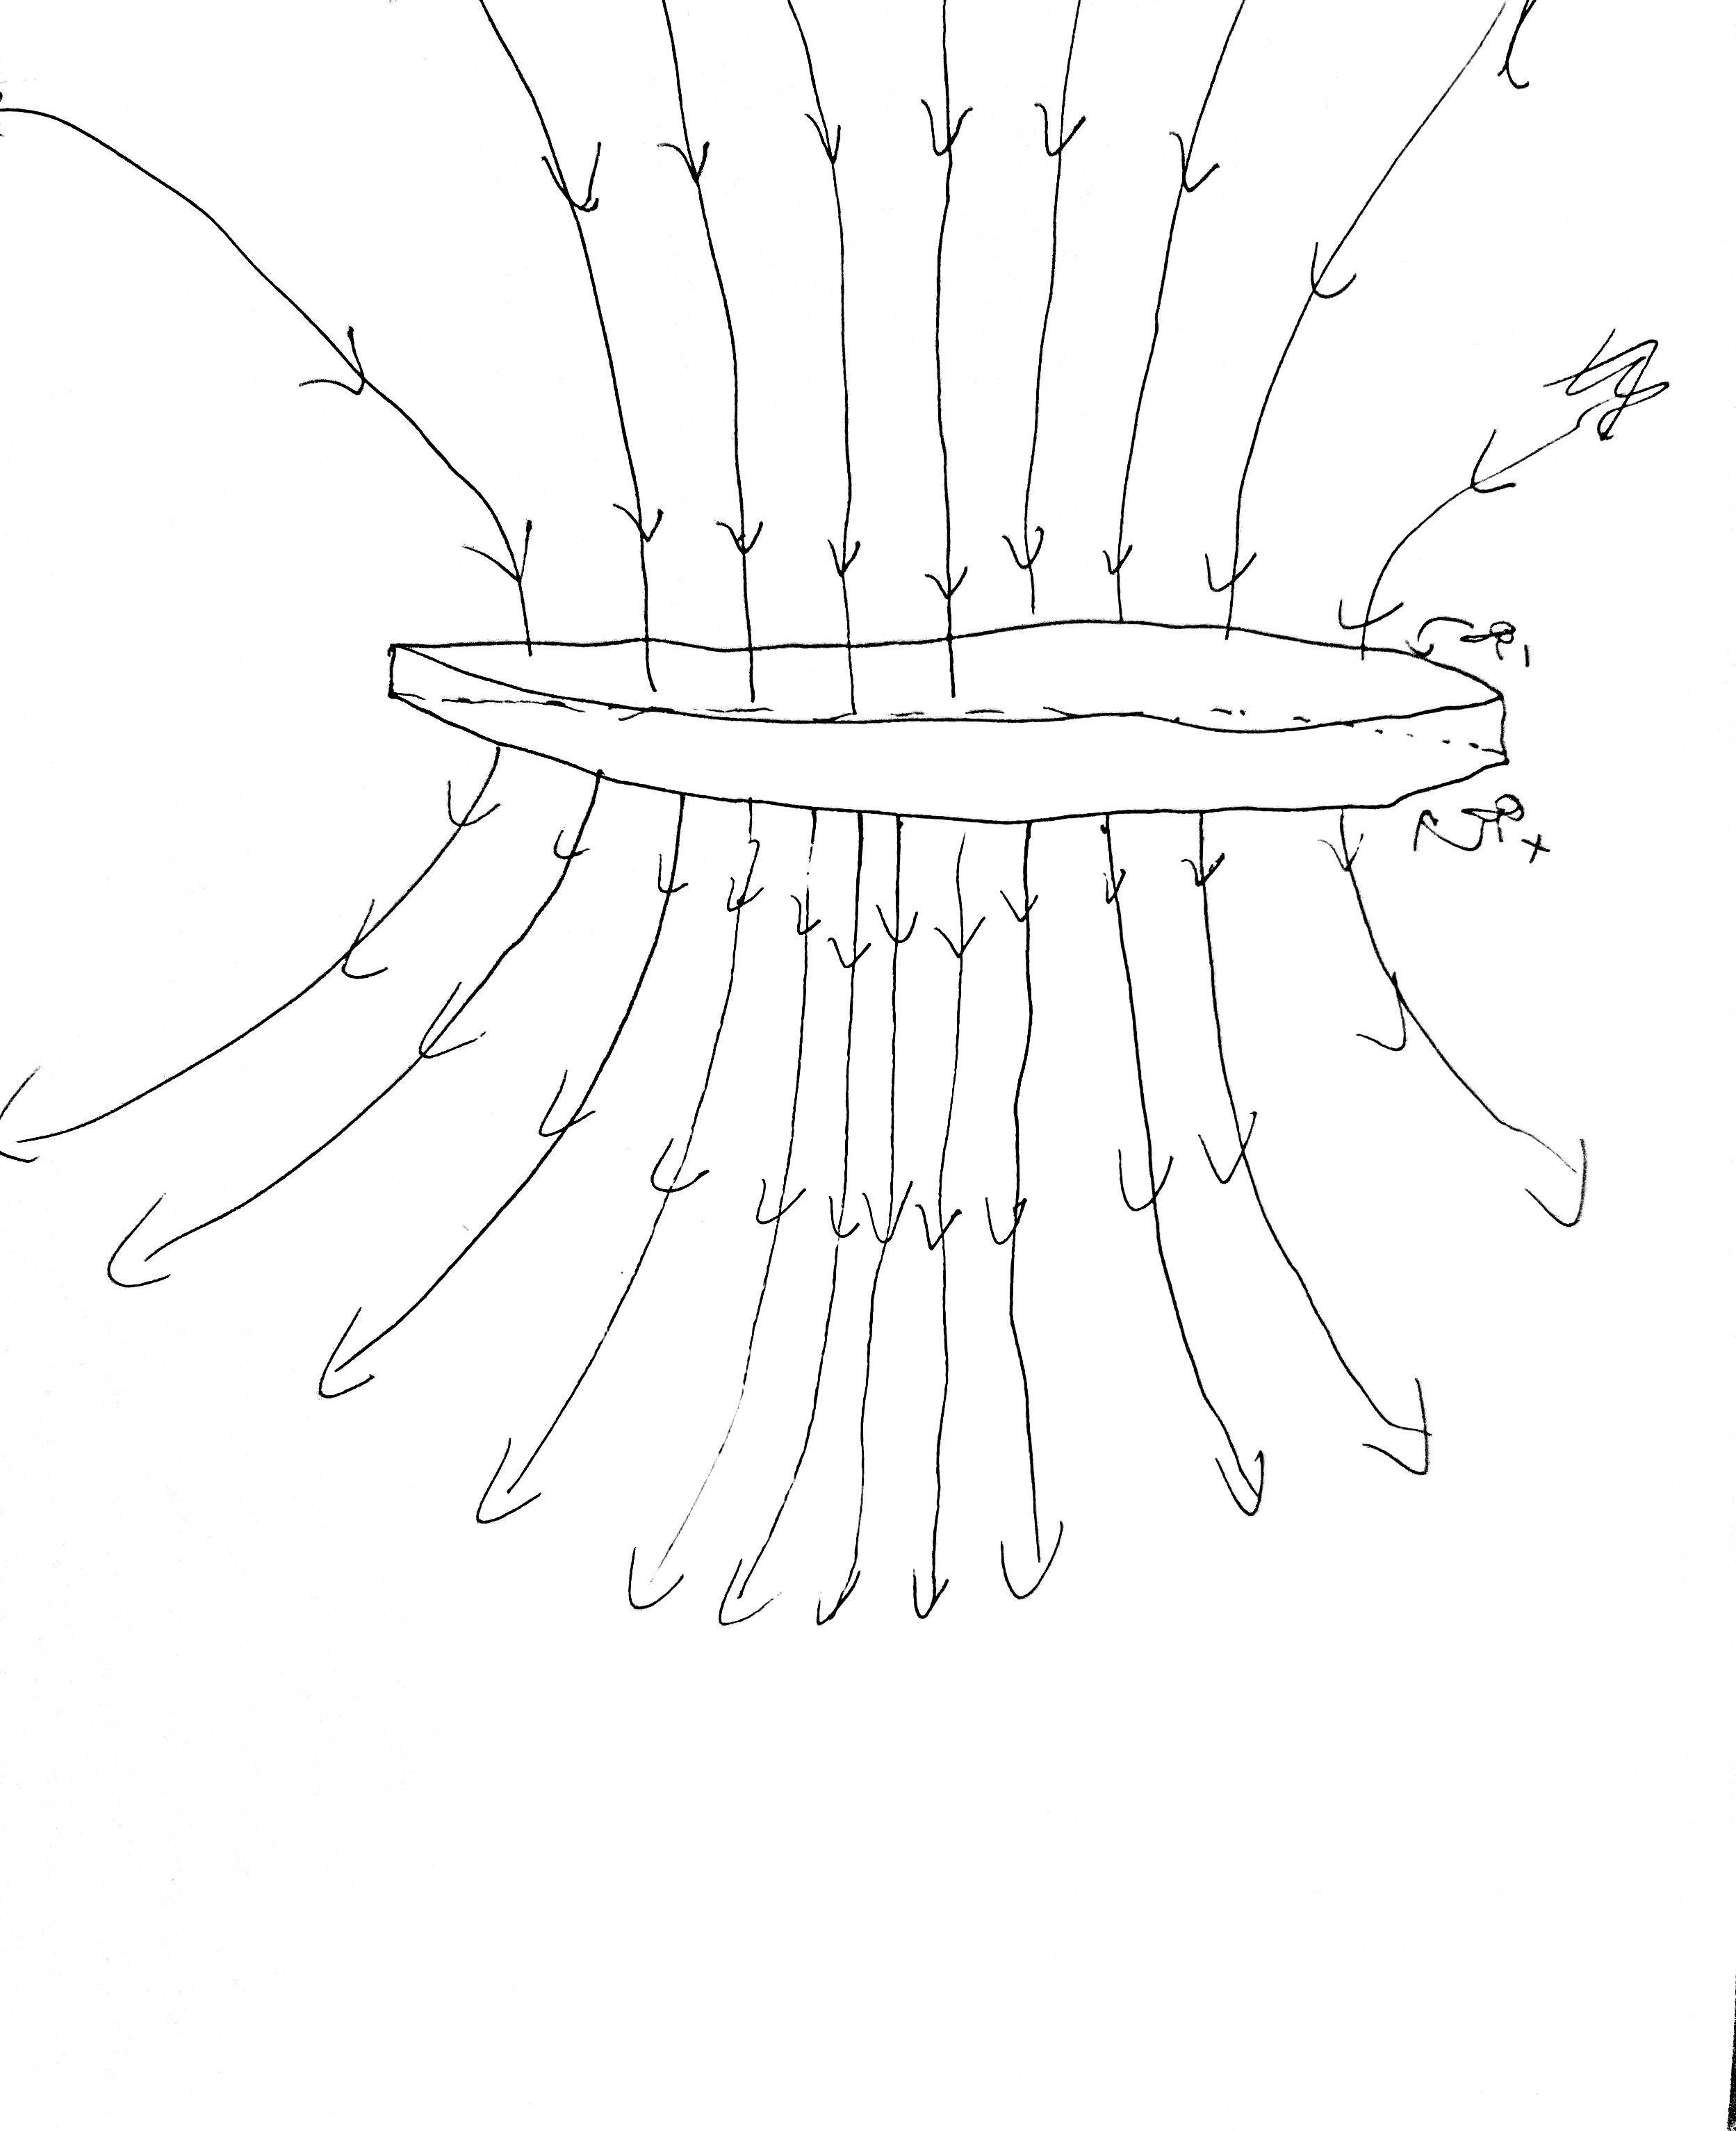
\includegraphics[scale=0.1, angle=90]{plot.jpg}\]

\section*{4a}
We apply the integral form of Gauss's law to find the displacement, since the problem exhibits spherical symmetry. Taking a Gaussian surface as a sphere centered on the charge,
\[\int_S\vec{D}\cdot d\vec{A}={\rho_{f}}\Rightarrow 4\pi r^2|\vec{D}|=Q\Leftrightarrow |\vec{D}|=\frac{Q}{4\pi r^2}\Rightarrow \vec{D}=\frac{Q}{4\pi r^2}\hat{r}\]
Nothing in the above argument depends on the permittivity of the material, so this holds for all values of $r$ both inside and outside the sphere.

\section*{4b}
Since in linear materials $\vec{D}=\epsilon\vec{E}$, the electric field is bifurcated:
\[\vec{E}=\frac{1}{\epsilon}\vec{D}=\begin{cases}
    \frac{Q}{4\pi\epsilon r^2} & r < a \\
    \frac{Q}{4\pi\epsilon_0r^2} & r > a \\
  \end{cases}\]
Since $\epsilon=\epsilon_0(1+\chi_e)$, in terms of the given quantities this is
\[\vec{E}=\begin{cases}
    \frac{Q}{4\pi\epsilon_0(1+\chi_e)r^2} & r < a \\
    \frac{Q}{4\pi\epsilon_0 r^2} & r > a\\
  \end{cases}\]

\section*{4c}
The boundary conditions for the displacement are \[D_{\textrm{above}}^\perp-D_{\textrm{below}}^\perp=\sigma_f\] and
\[\vec{D}_{\textrm{above}}^\parallel-\vec{D}_{\textrm{below}}^\parallel=\vec{P}_{\textrm{above}}^\parallel-\vec{P}_{\textrm{below}}^\parallel\]Since there is no free charge on the surface of the dielectric sphere, $D_{\textrm{above}}^\perp=D_{\textrm{below}}^\perp$, which holds since the perpendicular component $\frac{Q}{4\pi r^2}$ is continuous at $r=a$ (since $a\neq 0$).

Because by intuition the electric field, to which the polarization is proportional in linear materials, is directed radially outward, there is no parallel component to the polarization. This implies the perpendicular component of the displacement is continuous, which holds since $\vec{D}$ is continuous.

\section*{5}
Since intuitively the magnetic field may be expected to be tangent to circles concentric with the wire, we apply the integral form of Ampere's law on such loops. We use the $(r,\theta,z)$ cylindrical coordinate convention.
Outside the wire, this is simple, since the whole current flows through the loop:
\[\int_C\vec{B}\cdot d\vec{l}=\mu_0 I\Rightarrow 2\pi r|\vec{B}|=\mu_0 I\Leftrightarrow |\vec{B}|=\frac{\mu_0 I}{2\pi r} \Rightarrow \vec{B}=\frac{\mu_0I}{2\pi r}\hat{\theta}\]
The last implication is drawn from the right-hand rule; if the current is in the positive $z$ direction, the magnetic field will circulate counterclockwise, which is the positive $\theta$ direction.
Inside the wire, the proportion of current through the loop to the whole wire is that of the areas of the loop to the cross-section of the wire, i.e.
\[I_{enc}=\frac{\pi r^2}{\pi a^2}I=\frac{r^2}{a^2}I\]
Save for that, the argument is the same, so
\[2\pi r|\vec{B}|=\mu_0\frac{r^2}{a^2}I\Leftrightarrow |\vec{B}|=\frac{\mu_0rI}{2\pi a^2}\Rightarrow \vec{B}=\frac{\mu_0rI}{2\pi a^2}\hat{\theta}\]
In summary,
\[\vec{B}=\begin{cases}
    \frac{\mu_0 rI}{2\pi a^2}\hat{\theta} & r < a \\
    \frac{\mu_0 I}{2\pi r}\hat{\theta} & r > a
  \end{cases}\]

\section*{6a}
The bound volume current is defined as
\[\vec{J}_b=\nabla\times\vec{M}=\frac{1}{s}\left(\frac{\partial}{\partial s}(s\vec{M}_\phi)-\frac{\partial \vec{M_s}}{\partial \phi}\right)\hat{z}=4ks^2\hat{z  }\]
The bound surface current is, since the magnetization is everywhere perpendicular to the surface unit normal vector (which equals $\hat{r}$),
\[\vec{K}_b=\vec{M}\times\hat{n}=|\vec{M}(s=R)|(\hat{\phi}\times\hat{r})=-kR^3\hat{z}\]

\section*{6b}
All of the currents are (anti)parallel to $\hat{z}$, so we take as Amperian loops circles concentric with the cylinder lying in planes with normal vectors parallel to $\hat{z}$. Now we apply the integral form of Ampere's law for magenetic fields.

Outside the cylinder, the total enclosed current may be found by integrating the bound currents over the regions on which they are defined so that the result ``makes sense'' as a current:
\[I_{enc}=\int\vec{J}_b\cdot d\vec{A}+\int\vec{K}_b\cdot d\vec{l}=\int_0^{2\pi}\int_0^R4ks^2sdsd\phi+2\pi R(-kR^3)=2\pi k R^4-2\pi kR^4=0\]
This implies $\vec{B}=0$ in this region, since $\nabla\times \vec{B}=0$ and $\nabla\cdot \vec{B}=0$ are only satisfied simultaneously by the zero vector field.

Inside the cylinder, the process is similar, but there is no bound surface current enclosed by the loops and the integral for the bound volume current stops short of $R$.
\[I_{enc}=\int\vec{J}_b\cdot d\vec{A}=\int_0^{2\pi}\int_0^s4ks^2sdsd\phi=2\pi k s^4\]
Accordingly, the magnetic field isn't zero, but satisfies
\[\int_C\vec{B}\cdot d\vec{l}=\mu_0I_{enc}\Rightarrow 2\pi s|\vec{B}|=2\pi \mu_0ks^4\Leftrightarrow |\vec{B}|={\mu_0ks^3}\Rightarrow\vec{B}=\mu_0ks^3\hat{\phi}\]

\section*{6c}
The only currents in this problem are bound currents due to magnetization, i.e. there are no free currents. Since Ampere's law for the $\vec{H}$ field involves only the free current, $\vec{H}=0$ everywhere; once again, this is because $\nabla\times \vec{H}=0$ and $\nabla\cdot \vec{H}=0$ is satisfied by only the zero vector. This means you're evil for making us do $\vec{B}$ first; with this result we can deduce $\vec{B}=\mu_0\vec{M}$ immediately!

\section*{6d}
The two boundary conditions on $\vec{H}$ are
\[H_{\textrm{above}}^\perp-H_{\textrm{below}}^\perp=-(M_{\textrm{above}}^\perp-M_{\textrm{below}}^\perp)\]
and
\[\vec{H}_{\textrm{above}}^\parallel-\vec{H}_{\textrm{below}}^\parallel=\vec{K}_f\times\hat{n}\]
Since $\vec{M}$ is parallel to the surface and there is no free charge, both of the left-hand sides ought to be zero. Which they are, since $\vec{H}$ is zero everywhere.


\end{document}
%%% Local Variables:
%%% mode: latex
%%% TeX-master: t
%%% End:
